%Our click model is designed for CTR prediction of display advertising. The observations of this application are Users' profile information, Ads' static attributes, and Users' behavior history. Different from the sponsored search, users come into display advertising system without clear target. Thus we wish to mining users' interest from the context information and estimate the CTR of each display accurately.
\section{深度兴趣网络}\label{sec:opa}

与赞助搜索不同，用户进入展示广告系统时并没有明确表达的意图。
构建 CTR 预测模型时，需要有效方法从丰富的历史行为中提取用户兴趣。
描述用户和广告的特征是广告系统 CTR 建模的基本元素。
合理使用这些特征并从中挖掘信息至关重要。

\subsection{特征表征}
工业 CTR 预测任务中的数据大多呈多组类别形式，例如 [weekday=Friday, gender=Female, \\ visited$\_$cate$\_$ids=$\{$Bag,Book$\}$, ad$\_$cate$\_$id=Book]，
通常会通过编码转换为高维稀疏二值特征 \cite{deep_crossing,widedeep,ftrl}。
在数学上，第 $i$ 个特征组的编码向量形式化为 $\textbf{t}_i \in R^{K_i}$。$K_i$ 表示特征组 $i$ 的维度，即特征组 $i$ 包含 $K_i$ 个唯一 id。
$\textbf{t}_i[j]$ 是 $\textbf{t}_i$ 的第 j 个元素，且 $\textbf{t}_i[j] \in \{0,1\}$。$\sum_{j=1}^{K_i} \textbf{t}_i[j]=k$。
当 $k=1$ 时，向量 $\textbf{t}_i$ 表示 one-hot 编码；当 $k>1$ 时，表示 multi-hot 编码。
随后，一个样本可以按组表示为 $\bs{x} = [\bs{t}_1^T, \bs{t}_2^T,...\bs{t}_M^T]^T$，其中 $M$ 为特征组数量，$\sum_{i=1}^{M}K_i = K$，$K$ 为整个特征空间的维度。
通过这种方式，上述包含四组特征的样本可表示为：
%\begin{equation}
\[
%  \underbrace{a + \overbrace{b+\cdots}^{{}=t}+z}_{\text{total}} ~~ a + {\overbrace{b+\cdots}^{126}+z
\underbrace{[0,0,0,0,1,0,0]}_{\text{weekday=Friday}} ~ \underbrace{[0,1]}_{\text{gender=Female}} ~ \underbrace{[0,..,1,...,1,...0]}_{\text{visited\_cate\_ids=\{Bag,Book\}}} 
~ \underbrace{[0,..,1,...,0]}_{\text{ad\_cate\_id=Book}}
\]
%\end{equation}

表 \ref{table_feature_set} 描述了我们系统中使用的完整特征集。
它由四类特征组成，其中用户行为特征通常是 multi-hot 编码向量，并包含丰富的用户兴趣信息。
需要注意的是，在我们的设置中没有组合特征。我们使用深度神经网络捕获特征之间的交互。

\begin{table}
\caption{阿里巴巴展示广告系统中使用的特征集统计。特征按组由稀疏二值向量组成。} % The dimensionality of fine-grained $goods\_ids$ feature scales up to $10^9$.}
\centering
\resizebox{0.47\textwidth}{!}{%
\label{table:fea-table}
\begin{tabular}{llccc}
\toprule
Category & Feature Group & Dimemsionality & Type & \#Nonzero Ids per Instance\\ \toprule
\multirow{3}{7em}{User Profile Features }
& gender & 2 &  one-hot & 1  \\ \cline{2-5}
& age\_level & $\sim 10$ &  one-hot & 1  \\ \cline{2-5}
& ... & ... & ... & ...  \\ \midrule

\multirow{4}{7em}{User Behavior Features}
& visited\_goods\_ids& $\sim 10^9$ &  multi-hot & $\sim 10^3$  \\ \cline{2-5}
& visited\_shop\_ids& $\sim 10^7$ &  multi-hot & $\sim 10^3$  \\ \cline{2-5}
& visited\_cate\_ids& $\sim 10^4$ &  multi-hot & $\sim 10^2$  \\\midrule

\multirow{4}{7em}{Ad Features }
& goods\_id & $\sim 10^7$ &  one-hot & 1  \\ \cline{2-5}
& shop\_id & $\sim 10^5$ &  one-hot & 1  \\ \cline{2-5}
& cate\_id & $\sim 10^4$ &  one-hot & 1   \\ \cline{2-5}
& ... & ... & ... & ...  \\ \midrule

\multirow{3}{7em}{Context Features }
& pid & $\sim 10$ &  one-hot & 1  \\ \cline{2-5}
& time & $\sim 10$ &  one-hot & 1  \\ \cline{2-5}
& ... & ... & ... & ...  \\ \bottomrule
\end{tabular}}
\label{table_feature_set}
\end{table}


\begin{figure*}[!t]
\centering
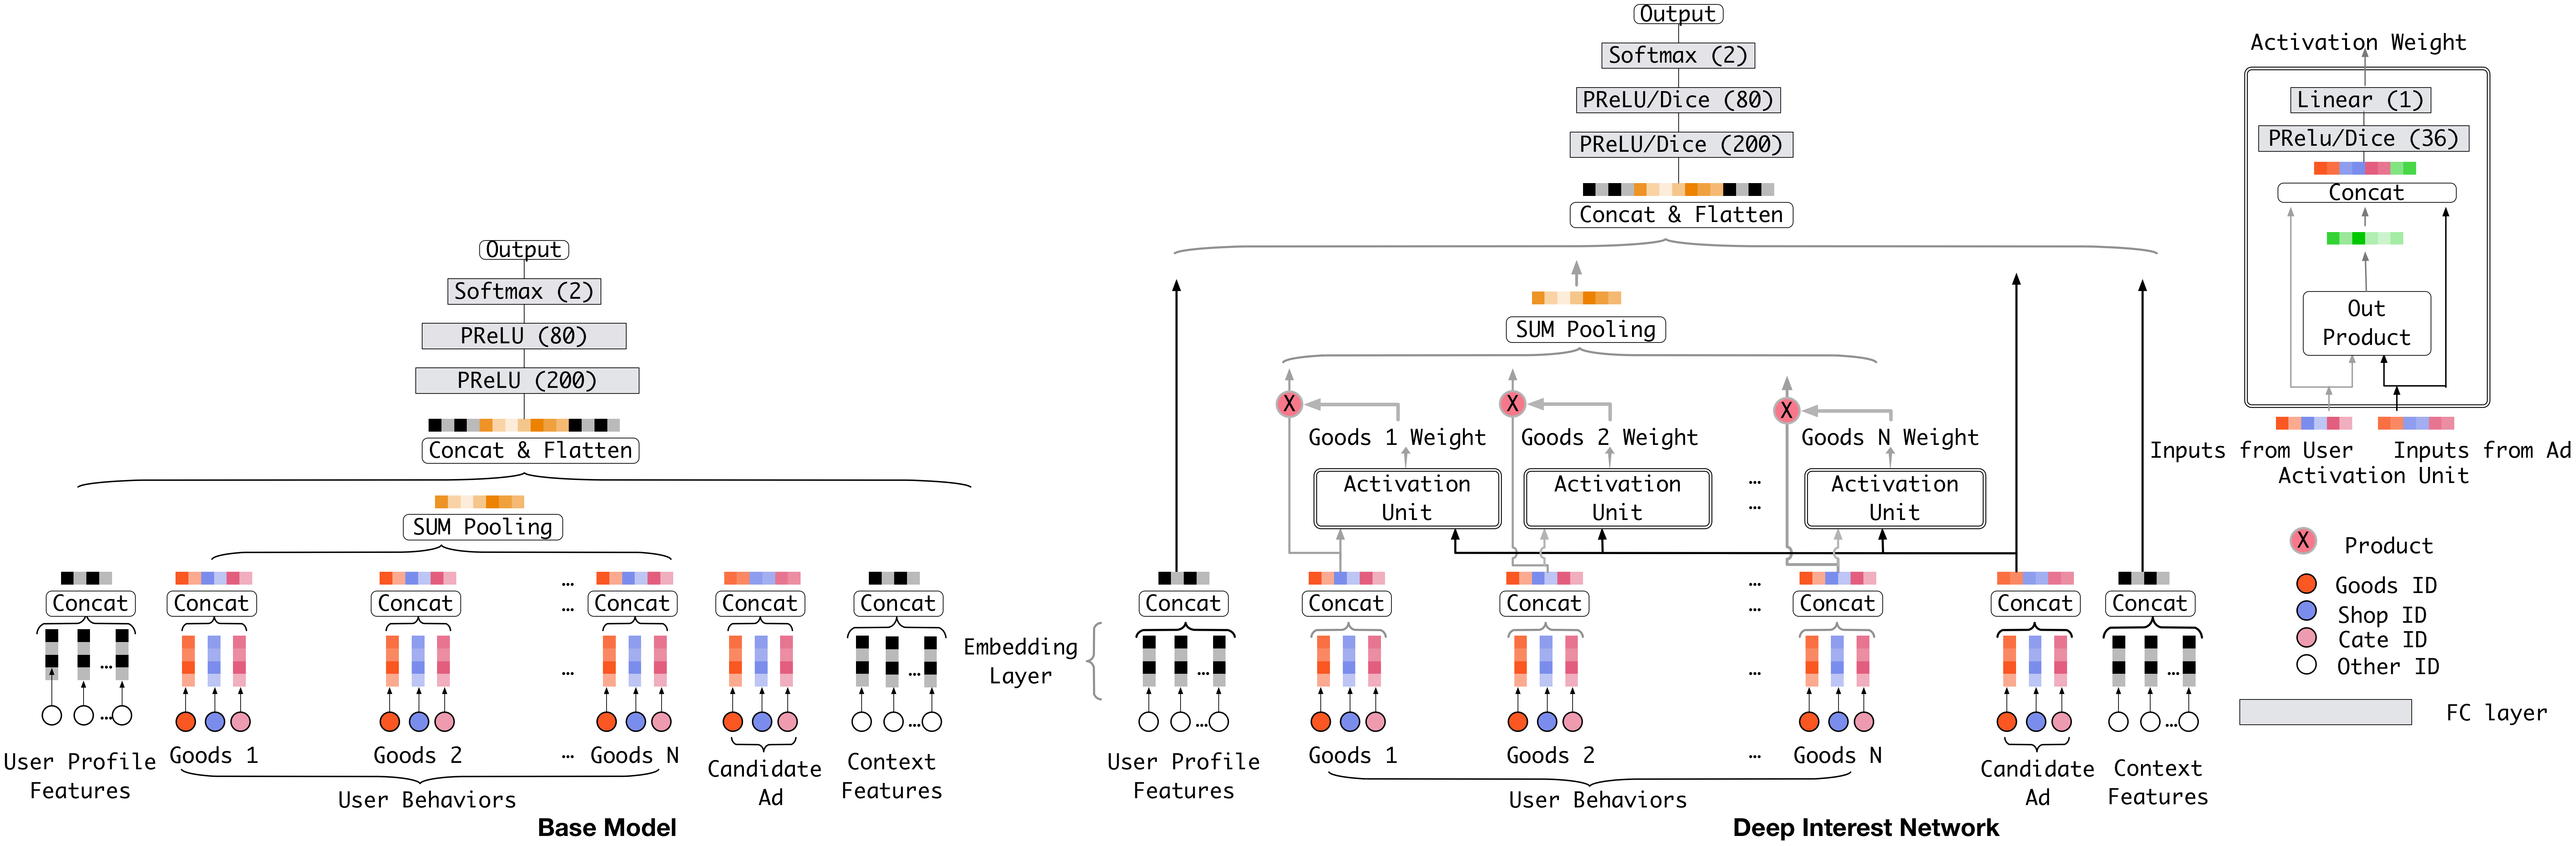
\includegraphics[height=7in, width=7in,keepaspectratio]{images/omni/DIN_new.png}
\caption{网络架构。左侧展示基础模型 (Embedding\&MLP) 的网络。属于同一商品的 cate\_id、shop\_id 和 goods\_id 的 embedding 被拼接起来，用于表示用户行为中的一个访问商品。右侧是我们提出的 DIN 模型。它引入局部激活单元，使用户兴趣表征能够针对不同候选广告自适应变化。}
\label{model_arch}
\end{figure*}


\subsection{基础模型 (Embedding\&MLP)}
\label{sec:basemodel}
%Following the popular model structure introduced in \cite{deep_crossing,widedeep,youtube:recommend}, we design our base model as shown in the left of Fig.\ref{model_arch}.
大多数流行模型结构 \cite{deep_crossing,widedeep,youtube:recommend} 共享相似的 Embedding\&MLP 范式，本文将其称为基础模型，如图 \ref{model_arch} 左侧所示。它由几个部分组成：
%It follows the embedding\&MLP architecture. %, with all the parameters trained in the end-to-end manner.
\paragraph{\textbf{Embedding 层}} 由于输入是高维二值向量，embedding 层用于将其转换为低维稠密表征。
%Let $\bs{t}_i\in \mathbb{R}^{K_i}$ represent the feature vector of i-th group in Table \ref{table_feature_set}. 
%Then one instance can be represent as $\bs{x} = [\bs{t}_1^T, \bs{t}_2^T,...\bs{t}_M^T]^T$ in a group-wise manner, where $M$ is number of feature groups, $\sum_{i=1}^{M}K_i = K$, $K$ is dimensionality of the entire feature space. 
对于 $\bs{t}_i$ 的第 $i$ 个特征组，令 $\mathrm{W}^i = [w_1^i,...,w_j^i, ..., w_{K_i}^i] \in\mathbb{R}^{D \times K_i}$ 表示第 $i$ 个 embedding 字典，其中 $w_j^i \in R^D$ 是维度为 $D$ 的 embedding 向量。
%Given instance of $\bs{x} = [\bs{t}_1^T, \bs{t}_2^T,...\bs{t}_M^T]^T$.
embedding 操作遵循查表机制，如图 \ref{model_arch} 所示。
\begin{itemize}
\item 如果 $\bs{t}_i$ 是 one-hot 向量，且第 j 个元素 $\bs{t}_i[j]=1$，则 $\bs{t}_i$ 的 embedding 表征是单个 embedding 向量 $\bs{e}_i = w_j^i$。
\item 如果 $\bs{t}_i$ 是 multi-hot 向量，且 $\bs{t}_i[j]=1 ~\text{for}~ j \in \{i_1, i_2, ..., i_k\} $，则 $\bs{t}_i$ 的 embedding 表征是一组 embedding 向量：$\{\bs{e}_{i_1}, \bs{e}_{i_2},...\bs{e}_{i_k}\} = \{w_{i_1}^i, w_{i_2}^i, ...w_{i_k}^i\}$。
\end{itemize}



\paragraph{\textbf{Pooling 层和 Concat 层}}
注意，不同用户拥有不同数量的行为。因此，multi-hot 行为特征向量 $\bs{t}_i$ 中非零值的数量会随样本变化，导致对应 embedding 向量列表的长度可变。
由于全连接网络只能处理定长输入，常见做法 \cite{widedeep,youtube:recommend} 是通过 pooling 层将 embedding 向量列表转换为定长向量：
\begin{equation}
\label{eq:pooling}
\bs{e}_i = \text{pooling}(\bs{e}_{i_1}, \bs{e}_{i_2},...\bs{e}_{i_k}).	
\end{equation}
最常用的两种 pooling 层是 sum pooling 和 average pooling，它们对 embedding 向量列表执行逐元素求和或求平均操作。

embedding 层和 pooling 层都按组操作，将原始稀疏特征映射为多个定长表征向量。
随后，将所有向量拼接起来，得到该样本的整体表征向量。

\paragraph{\textbf{MLP}} 给定拼接后的稠密表征向量，全连接层用于自动学习特征组合。
近期提出的方法 \cite{widedeep,DeepFM,PNN} 关注 MLP 结构设计，以更好地提取信息。\par
\paragraph{\textbf{损失}}基础模型使用的目标函数是负对数似然函数，定义如下：
\begin{equation}
    L= - \frac{1}{N} \sum_{(\bs{x},y)\in\mathcal{S}} (y\log p(\bs{x}) + (1-y)\log(1-p(\bs{x}))),
\end{equation}
其中 $\mathcal{S}$ 是大小为 $N$ 的训练集，$\bs{x}$ 是网络输入，$y\in \{0,1\}$ 是标签，$p(\bs{x})$ 是网络经过 softmax 层后的输出，表示样本 $\bs{x}$ 被点击的预测概率。


\subsection{深度兴趣网络结构}

在表 \ref{table_feature_set} 的所有特征中，用户行为特征至关重要，并在电商应用场景中的用户兴趣建模中发挥关键作用。

基础模型通过对用户行为特征组中的所有 embedding 向量进行 pooling，获得用户兴趣的定长表征向量，如式 (\ref{eq:pooling}) 所示。对于给定用户，无论候选广告是什么，该表征向量都保持不变。
通过这种方式，维度有限的用户表征向量会成为表达用户多样化兴趣的瓶颈。
为了使其具备足够能力，一个简单方法是扩展 embedding 向量的维度，但这会显著增加学习参数规模。
在训练数据有限时，这会导致过拟合，并增加计算和存储负担，而工业级在线系统可能无法承受这些开销。

%As discussed above, when visiting e-commerce sites, users are often interested in many kinds of goods. 
%In other words, user interests are diverse.  
%However, it is known that users are often with diverse interests when visiting e-commerce sites. 
%Base model obtains the user interest vector by average pooling over the embedding of all behaviors. Thus base model obtains a same interest vector of users given different candidate ads for one user.
% In the base model, sums the embedding of all user behavior ids to obtain the user interest vector. The model obtains the same user % interest vector when predicts different candidate ad for one user.
%In order to embed diverse user interests in this vector, one easy method is expanding the dimension to make it capable enough to contain information of different interests. 
%Unfortunately, high dimension of embedding vectors will increase the size of learning parameters heavily.
%It will lead to overfitting under limited training data and add the burden of computation and storage, which may not be tolerated for an industrial online system.

是否存在一种优雅方式，能够在有限维度下用一个向量表示用户的多样化兴趣？
用户兴趣的局部激活特征启发我们设计了一种名为深度兴趣网络 (DIN) 的新模型。
设想第 \ref{sec:bg} 节中提到的年轻母亲访问电商网站时，看到展示的新手提包很可爱并点击了它。
我们分析这一点击行为的驱动力。
所展示的广告通过软搜索她的历史行为，并发现她近期浏览过相似的托特包和皮质手提包商品，从而命中了这位年轻母亲的相关兴趣。
换言之，与展示广告相关的行为对点击动作有很大贡献。
DIN 通过关注相对于给定广告的局部激活兴趣表征来模拟这一过程。
DIN 不使用同一个向量表达用户的全部多样化兴趣，而是考虑历史行为相对于候选广告的相关性，自适应计算用户兴趣表征向量。
该表征向量会随广告不同而变化。

图 \ref{model_arch} 右侧展示了 DIN 的架构。
与基础模型相比，DIN 引入了新设计的局部激活单元，并保持其他结构不变。具体而言，激活单元应用于用户行为特征，在给定候选广告 $A$ 时执行加权求和池化，以自适应计算用户表征 $\bs{v}_U$，如式 (\ref{eq:attention}) 所示。


%By simulating this process, we   
%Instead of focusing on a global representation vector, we actually only need to pay attention to the representation of locally related interests given a candidate ad.  
%In this way, representation vector of user interest is calculated adaptively given $\prec$user, ad$\succ$ pair. 
%That is, it varies over different candidate ads.  
%Then user vector only needs to represent related interest when faced different candidate ad, which is within the ability of a vector with appropriate dimension. \par
%For different candidate ads, we want our model to find related part of interests automatically. \par
%This candidate specific interest vector can be realized by attention mechanism\cite{bengio:attention}, which derive from neural machine translation.
%Under this consideration, we design a novel model named deep interest network(DIN), to better capture the characteristic of user behavior data and help improving the expressive ability of model under limited embedding dimension. 
%It is illustrated in the right of Fig.\ref{model_arch}.
%Compared with base model, DIN introduces a new designed activation unit and maintains the other net structures the same.  

%Specifically, activation unit is applied on the user behavior feature groups, which performs as a weighted average pooling to adaptively calculate user representation $\bs{v}_U$ given a candidate ad $A$, as shown in Eq.(\ref{eq:attention})
{
%\setlength\abovedisplayskip{1pt}
%\setlength\belowdisplayskip{1pt}
\begin{small}
\begin{equation}
\begin{split}
\label{eq:attention}
\bs{v}_U(A) = f(\bs{v}_A,\bs{e}_1,\bs{e}_2,..,\bs{e}_H) & = \sum_{j=1}^H a(\bs{e}_j,\bs{v}_A) \bs{e}_j = \sum_{j=1}^H \bs{w}_j \bs{e}_j,
\end{split}
\end{equation}
\end{small}
}
其中 $\{\bs{e}_1, \bs{e}_2, ..., \bs{e}_H\}$ 是用户 $U$ 的行为 embedding 向量列表，长度为 $H$，$\bs{v}_A$ 是广告 $A$ 的 embedding 向量。通过这种方式，$\bs{v}_U(A)$ 会随广告不同而变化。$a(\cdot)$ 是一个前馈网络，其输出作为激活权重，如图 \ref{model_arch} 所示。除两个输入 embedding 向量外，$a(\cdot)$ 还加入它们的外积并输入后续网络，这是一种有助于相关性建模的显式知识。

式 (\ref{eq:attention}) 中的局部激活单元与 NMT 任务中发展的注意力方法 \cite{bengio:attention} 具有相似思想。
然而，与传统注意力方法不同，式 (\ref{eq:attention}) 放宽了 $\sum_i w_i = 1$ 约束，目的是保留用户兴趣强度。
也就是说，我们舍弃了对 $a(\cdot)$ 输出进行 softmax 归一化。
相反，$\sum_i w_i$ 的值在一定程度上被视为激活用户兴趣强度的近似。
例如，如果某个用户的历史行为中 90\% 是服装，10\% 是电子产品。
给定 T 恤和手机两个候选广告，T 恤会激活大多数属于服装的历史行为，并可能比手机得到更大的 $\bs{v}_U$ 值，即更高的兴趣强度。
传统注意力方法通过归一化 $a(\cdot)$ 的输出，会丢失 $\bs{v}_U$ 数值尺度上的分辨率。
%Taking the original output of $a(\cdot)$  as activation score can be a simple way to maintain the intensity of interest, which helps making use of user historical behavior data more sufficiently.


%Assume user U is interested in clothes and electronics, with the intensity to be 90\% and 10\% relatively. 
%This causes the historical behaviors of clothes occur more \textbf{frequently} than electronics for $U$.     
%Assume two candidate ads T-shirt and iphone are selected as candidates for $U$.
%Value of representation vector $\bs{v}_U$ given T-shirt will be larger than given iphone.
%Indeed, taking the original output of $a(\cdot)$  as activation weight can be a simple way to maintain the intensity of interest, which helps us making use of user historical behavior more sufficiently.

我们尝试过用 LSTM 以序列方式建模用户历史行为数据。
但它没有带来提升。
%But it makes little difference. 
不同于 NLP 任务中受语法约束的文本，用户历史行为序列可能包含多个并发兴趣。
这些兴趣之间的快速跳转和突然终止会使用户行为序列数据显得有噪声。
一个可能方向是设计特殊结构，以序列方式建模这类数据。
我们将其留作未来研究。


%Meanwhile, user behavior is not only affected by his diverse interests but also depends on the results our system display. 
%In our attempt, directly modeling user behavior sequence with RNNs shows little improvement.  
%This makes it difficult for directly deploying the RNNs to model user behavior sequence in e-commerce scenario.

%It's notable that the value of $\bs{v}_U$ given candidate ad that relates to \textbf{frequent} historical behavior is larger than others. 
%For example, if one user's historical behavior contains 80\% clothes and 20\% electronics. For candidate ads: T-shirt and phone, more historical behaviors get high attention score for T-shirt, which leads to the value of vector $\bs{v}_U$ computed for the user is larger for T-shirt than for phone. It means the value of vector can reflect the user's interest intensity. But traditional attention methods that use normalization with softmax on the output of $a$ to scale the value of $\bs{v}_U$ into the same range is not suitable in our scenario, which may lose the information of interest intensity. Instead, the original output of $a$ can maintain the intensity of interest, which helps us making use of user historical behavior more sufficiently.

%It seems to be natural to use RNNs for modeling user interest by taking the sequence of user behaviors as inputs. 
%However, we implement it and find no difference. 
%A possible explanation is that different from text that is under the constraint of grammar, the sequence of user historical behaviors contains concurrent multiple varying interests and may rapidly jump over these interests, which make the sequence data to be disordered and noisy. 
%We leave this for future research. 
%Meanwhile, user's behavior is not only affected by his diverse interests but also another factors such as the results our system display. Thus the information about sequence in e-commerce scenario is much weaker than that in text.
 

%The use of attention makes users' diverse interest be captured. Further, these diversity interest can be local activated when predict one specific candidate ad.
%In all, DIN designs the activation unit to follow local activation structure and weighted sum pooling to follow diversity structure.
%To the best of our knowledge, DIN is the first model which follows both of the two structures of user behavior data in CTR prediction tasks at the same time.
%\subsection{Mini-batch Aware Regularization Technique}

\section{训练技术}
在阿里巴巴广告系统中，商品和用户数量规模达到数亿。
%There are billion kinds of goods in Alibaba, and our advertising system needs to serve more than hundred million users one day.
实际中，使用大规模稀疏输入特征训练工业级深度网络具有很大挑战。
本节介绍两项在实践中被证明有帮助的重要技术。

\subsection{Mini-batch Aware 正则化}

%In order to capture more specific interests of users, we typically introduce billions of fine-grained ids to describe the users' behaviors. These sparse and high dimensional features may lead to severe overfitting problem.
%{\EDIT why these feature would cause overfitting?(1 more parameter ; 2 less times)}
%to capture user interest detailly. \par
%Not surprisingly, overfitting problem is encountered while training our model with large scale parameters and sparse inputs.
%In experiment, with addition of fine-grained user visited $good\_ids$ feature, model performance falls rapidly after the first epoch.\par
%It is known that internet-scale user behavior data follows the long-tail law, that is, lots of feature ids occur a few times in the training samples, while little of them occur many times.
%This inevitably introduces noise into the training process and intensifies overfitting.
%An easy way to reduce overfitting is to filter out those low-frequency feature ids, which can be viewed as manual regularization.
%However, such frequency based filter is quite rough in terms of information loss and threshold setting.
%Many methods have been proposed to reduce overfitting, such as $\ell_2$ and $\ell_1$ regularization \cite{lasso}, and Dropout \cite{dropout}. 
%However, merely of them are suitable for training network with sparse inputs and billions of parameters.

%Practically overfitting problem is encountered while training industrial networks with large scale sparse input features.
过拟合是训练工业级网络的关键挑战。
例如，加入细粒度特征后，如维度为 6 亿的 $\textsl{goods\_ids}$ 特征，包括表 \ref{table_feature_set} 中描述的用户 $visited\_goods\_ids$ 和广告 $goods\_id$，如果训练时不使用正则化，模型性能会在第一个 epoch 后迅速下降，如后文第 \ref{sec:reg} 节图 \ref{fig:adaptive_reg} 中的深绿色曲线所示。
对于稀疏输入且包含数亿参数的网络，直接使用传统正则化方法并不现实，例如 $\ell_2$ 和 $\ell_1$ 正则化。
以 $\ell_2$ 正则化为例。
在没有正则化的基于 SGD 的优化方法中，每个 mini-batch 只需要更新出现的非零稀疏特征参数。
然而，加入 $\ell_2$ 正则化后，每个 mini-batch 都需要在全部参数上计算 L2-norm，这会产生极重的计算开销，当参数规模达到数亿时不可接受。
%Original $\ell_2$ regularization needs to calculated L2-norm over the whole parameters on each mini-batch, which leads to extremely heavy computations and is unacceptable in our situation. 

\begin{figure}[!ht]
%\setlength{\belowcaptionskip}{-0.5cm}
\centering
%\includegraphics[height=4.5in, width=5in,keepaspectratio]{images/omni/system}
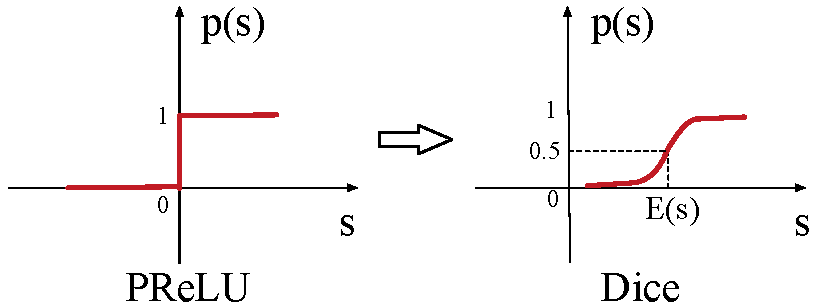
\includegraphics[height=1.8in, width=2.2in,keepaspectratio]{images/omni/dice_activation}
\caption{PReLU 和 Dice 的控制函数。}
\label{figure_dice}
\vspace{-0.4cm}
\end{figure} 


本文提出了一种高效的 mini-batch aware 正则化器，它只对每个 mini-batch 中出现的稀疏特征参数计算 L2-norm，从而使计算可行。
事实上，CTR 网络的大部分参数来自 embedding 字典，也正是它带来了沉重计算的困难。
令 $\bs{\mathrm{W}}\in\mathbb{R}^{D\times K}$ 表示整个 embedding 字典的参数，其中 $D$ 是 embedding 向量维度，$K$ 是特征空间维度。
在样本上展开 $\bs{\mathrm{W}}$ 的 $\ell_2$ 正则化：
%\begin{equation}
%\label{eq:batch}
%\sum_{i=1}^{n_{dj}} \frac{I_{id}}{n_{dj}}w_d^2
%\end{equation}
\begin{footnotesize}
\begin{equation}
\begin{split}
\label{eq:batch}
L_2(\bs{\mathrm{W}}) &= \|\bs{\mathrm{W}}\|_2^2 = \sum_{j=1}^{K}\|\bs{w}_j\|_2^2 = \sum_{(\bs{x},y)\in\mathcal{S}}\sum_{j=1}^{K} \frac{I(\bs{x}_j\neq0)}{n_{j}}\|\bs{w}_j\|_2^2,
\end{split}
\end{equation}
\end{footnotesize}
其中 $\bs{w}_j\in\mathbb{R}^{D}$ 是第 $j$ 个 embedding 向量，
%which corresponding to the number of feature IDs in our applications.
$I(\bs{x}_j\neq0)$ 表示样本 $\bs{x}$ 是否具有特征 id $j$，$n_j$ 表示特征 id $j$ 在所有样本中的出现次数。%Here we use $I(\cdot)$ as the indicator function.
%When applying the gradient descent optimization on mini-batches, the regularization is transformed into
式 (\ref{eq:batch}) 可以按 mini-batch aware 方式转换为式 (\ref{eq:minibatch})：
\begin{small}
\begin{equation}
\label{eq:minibatch}
L_2(\bs{\mathrm{W}}) = \sum_{j=1}^{K}\sum_{m=1}^{B}\sum_{(\bs{x},y)\in\mathcal{B}_m}\frac{I(\bs{x}_j\neq 0)}{n_{j}}\|\bs{w}_j\|_2^2,
\end{equation}
\end{small}
其中 $B$ 表示 mini-batch 的数量，$\mathcal{B}_m$ 表示第 $m$ 个 mini-batch。
%To simplify the computation, 
令 $\alpha_{mj} = \max_{(\bs{x},y)\in\mathcal{B}_m} I(\bs{x}_j\neq0)$
%{\small
%\begin{equation}
%\alpha_{mj} = \max_{(\bs{x},y)\in\mathcal{B}_m} I(\bs{x}_j\neq0),
%\end{equation}}
表示 mini-batch $\mathcal{B}_m$ 中是否至少有一个样本包含特征 id $j$。
则式 (\ref{eq:minibatch}) 可以近似为：
\begin{small}
\begin{equation}
\label{eq:approx}
L_2(\bs{\mathrm{W}})\approx\sum_{j=1}^{K} \sum_{m=1}^{B}  \frac{\alpha_{mj}}{n_j}\|\bs{w}_j\|_2^2.
\end{equation}
\end{small}
通过这种方式，我们推导出了 $\ell_2$ 正则化的近似 mini-batch aware 版本。
对于第 $m$ 个 mini-batch，关于特征 $j$ 的 embedding 权重的梯度为：
%\begin{equation}	
%\scalebox{0.9}{
%\parbox{0.37\textwidth}{
%\begin{eqnarray}
%\begin{split}
%\bs{w}_j \leftarrow \bs{w}_j- \eta
%    \left[
%       \frac{1}{|\mathcal{B}_m|} \sum_{(\bs{x},y) \in \mathcal{B}_m} { \frac{\partial L(p(\bs{x}), y)}{\partial \bs{w}_j}
%       +\lambda \frac{\alpha_{mj}}{n_j}\bs{w}_j}
%    \right].
%\end{split}
%\end{eqnarray}
%}
%}
%\end{equation}
\begin{small}
\begin{equation}
\bs{w}_j \leftarrow \bs{w}_j- \eta
    \left[
       \frac{1}{|\mathcal{B}_m|} \sum_{(\bs{x},y) \in \mathcal{B}_m} { \frac{\partial L(p(\bs{x}), y)}{\partial \bs{w}_j}
       +\lambda \frac{\alpha_{mj}}{n_j}\bs{w}_j}
    \right],
\end{equation}
\end{small}
其中只有出现在第 $m$ 个 mini-batch 中的特征参数参与正则化计算。

%Different from the regularization in~\cite{difacto}, our approach imposes more penalty on long-tail features(which is hard to learn) of lower frequency than frequent $goods\_id$(which may reflect user interests confidently). 
%Experiments show that our approach outperforms other regularization methods, like dropout.




% let $w_j$ denotes the parameter in embedding layer,
%In common, the gradient of loss  $L(x; W)$ combined with $L_2(W)$ to the embedding layer's parameter $W_{jk}$(the embedding matrix for the kth id of feature $X_j$)is
%\begin{equation}
%\label{ada-reg}
%W_{jk} \leftarrow W_{jk} - \eta
%    \left[
%       \frac{1}{b} \sum_{(x_i,y_i) \in B} { \frac{\partial L(f(x_i), y_i)}{\partial W_{jk}} +\lambda W_{jk}}
%    \right]
%\end{equation}
%Where $B$ stands for mini-batch samples with size of $b$.  $\lambda$ is regularization parameter.

%Many methods have been proposed to reduce overfitting, such as $L_2$ and $L_1$ regularization \cite{lasso}, and Dropout \cite{dropout}.
%However, with sparse and high dimensional data,  CTR prediction task faces greater challenge.
%It is known that internet-scale user behavior data follows the long-tail law, that is, lots of feature ids occur a few times in the training samples, while little of them occur many times.
%This inevitably introduces noise into the training process and intensifies overfitting.
%
%%According to our experience,
%An easy way to reduce overfitting is to filter out those low-frequency feature ids, which can be viewed as manual regularization.
%However, such frequency based filter is quite rough in terms of information loss and threshold setting.
%Here we introduce an adaptive regularization method, in which we impose different regularization intensity on feature ids according to their occurrence frequency.
%On realizing this method, we apply frequency related L2-norm regularization to good ids that actually occur in current mini-batch.
%The last term brings to some problem, on the one hand, it has effect on $W_{jk}$ even if $x_{ij}$ is 0. On the one hand, it improves the consumption of computation; On the other hand, it will lead error director for the update of $w_{e_j}$.\par
%
%In order to avoid extra updating, we try to introduce one control unit to the update when one batch using one specific id.
%Denote that,
%\begin{equation}
%I_i = \left\{ \begin{array}{ll}
%1, & \exists  (x_j,y_j) \in B, s.t. \left[ x_j \right]_i \neq 0\\
%0, & \textrm{other wises}
%\end{array} \right.
%\end{equation}
%
%\begin{equation}
%\label{ada-reg}
%W_{jk} \leftarrow W_{jk} - \eta
%    \left[
%       \frac{1}{b} \sum_{(x_i,y_i) \in B} { \frac{\partial L(f(x_i), y_i)}{\partial W_{jk}} +\lambda W_{jk}I_i}
%    \right]
%\end{equation}
% While there is another problem, the update times for different frequent feature is different, which means the regularization on low frequent feature is weak, which violates the goal.\par
% Aiming to solve this problem, we design an adaptive regularization method, which applies different regularization intensity on feature ids according to their occurrence frequency.
%Let's analyze the gradient updating from the aspect of instance.
%Aiming to solving this problems, we design an adaptive regularization method, which imposes different regularization intensity on feature ids according to their occurrence frequency.\par
%Denote that,
%\begin{equation}
%I_i = \left\{ \begin{array}{ll}
%1, & \exists  (x_j,y_j) \in B, s.t. \left[ x_j \right]_i \neq 0\\
%0, & \textrm{other wises}
%\end{array} \right.
%\end{equation}

%\begin{equation}
%\label{ada-reg}
%W_{jk} \leftarrow W_{jk} - \eta
%    \left[
%       \frac{1}{b} \sum_{(x_i,y_i) \in B} { \frac{\partial L(f(x_i), y_i)}{\partial W_{jk}} +\lambda \frac{1}{n_i}W_{jk}I_i}
%    \right]
%\end{equation}
%where $n_i$ is frequency of feature $i$.\par


%The idea behind Eq.(\ref{ada-reg}) is to penalize low-frequency features and relax high-frequency features to control the gradient update variance.
%When b is set to 1, the update is equivalent to dividing regularization term of full batch update onto each sample. When mini batch size is large than 1, we still use $\lambda \frac{1}{n_i}$ as regular coefficient to avoid counting good id's frequency in current mini batch.

%% PLAN A
%A similar practice of adaptive regularization can be found in \cite{difacto} which sets regular coefficient to be proportional to feature frequency where they
%, as shown below:
%\begin{equation}
%\label{limu}
%w_i \leftarrow w_i - \eta
%    \left[
%       \frac{1}{b} \sum_{(x_j,y_j) \in B} { \frac{\partial L(f(x_j), y_j)}{\partial w_i} +\lambda n_iw_iI_i}
%    \right]
%\end{equation}
%However, in our dataset, training with regularization of Eq.(\ref{limu}) shows no obvious alleviation of overfitting. On the contrary, it slows down the convergence of training process. Eq.(\ref{limu}) applies greater penalty on high-frequency good ids than long-tail goods, while the former contributes more on both the metric and online income in our special e-commerce system. Besides, we also evaluate dropout technique and find slight improvement on overfitting.
%However, when we train DNN model on our display advertisement data using the above equation, we could not observe the alleviation of overfitting. On the contrary, it slows down the convergence of training process, because of greater penalty on high-frequency good ids. We have also tested the case in which all good ids share the same regular coefficient, in other words, regular coefficient has no relationship with item frequency. In that case, overfitting still exists and the speed of convergence also slows down.
%\end{comment}


\subsection{数据自适应激活函数}
%{\EDIT
%In order to make DIN to be more suitable for industrial-scale net sparse input, besides the design of net structure and choice of input, we propose a new activation function to accelerate the convergence.

%Industrial-scale dimensionality of sparse features and data size give challenges to the convergence for training deep networks. 
%To fit the data better, we propose a data adaptive activation function to help convergence.



PReLU \cite{ms:prelu} 是一种常用激活函数：
\begin{small}
\begin{equation}
f(s) = \begin{cases}
       s & \text{ if } s > 0  \\
       \alpha s & \text{ if } s \leq 0.
       \end{cases}
     = ~ p(s) \cdot s + (1-p(s))\cdot \alpha s,   
\end{equation}
\end{small}
其中 $s$ 是激活函数 $f(\cdot)$ 输入的一维，$p(s) = I(s>0)$ 是指示函数，用于控制 $f(s)$ 在 $f(s)=s$ 和 $f(s)=\alpha s$ 两个通道之间切换。第二个通道中的 $\alpha$ 是学习参数。
这里我们将 $p(s)$ 称为控制函数。图 \ref{figure_dice} 左侧绘制了 PReLU 的控制函数。
PReLU 采用值为 $0$ 的硬整流点，当各层输入服从不同分布时，这可能并不合适。
考虑到这一点，我们设计了一种新的数据自适应激活函数，命名为 \textsl{\textbf{Dice}}：
\begin{equation}
f(s) = p(s) \cdot s + (1-p(s))\cdot \alpha s, \ \ p(s) = \frac{1}{ 1 + e^{- \frac{s - E[s]}{\sqrt{Var[s] + \epsilon}}}}
\end{equation}
其控制函数绘制在图 \ref{figure_dice} 右侧。
在训练阶段，$E[s]$ 和 $Var[s]$ 是每个 mini-batch 中输入的均值和方差。
在测试阶段，$E[s]$ 和 $Var[s]$ 由数据上的移动平均 $E[s]$ 和 $Var[s]$ 计算得到。
$\epsilon$ 是一个很小的常数，在我们的实践中设为 $10^{-8}$。

Dice 可以看作 PReLU 的一种推广。
Dice 的核心思想是根据输入数据分布自适应调整整流点，其值设为输入均值。
此外，Dice 以平滑方式控制两个通道之间的切换。
当 $E(s)=0$ 且 $Var[s]=0$ 时，Dice 退化为 PReLU。



%The key idea of Dice is to adaptively adjust the rectifier point according to data, which is different from PReLU.
%Instead of using a hard rectifier based on whether y is larger than 0,
%Dice adjusts the rectifier point by portion of $p$ which contains information of the mean and variance of inputs.
%It can be viewed as a soft rectifier with two channel: $\alpha y$ and $y$. $p$ is a adaptive weight. 

%PReLU plays the role as the Leaky ReLU to avoid zero gradients \cite{Mass:Lrelu} while the $a_i$ is small.
%Previous research has shown that PReLU can improve accuracy while with a little extra risk of overfitting.
%However, in our application with large scale sparse inputs, training such industrial-scale network  still faces a lot of  challenges.
%All variants of ReLU choose $0$ as the rectifier point. 
%However a hard rectifier point may be not suitable as the distribution of each layers's input is different.
%To further improve the convergency and performance of our model, 
%Hence, we design a novel data adaptive activation function, which we name Dice:
%\begin{align}
%f(\bs{y}_{k}) & = \bs{a}_{(k)}(1 - \bs{p}_{k})\bs{y}_{k} + \bs{p}_{k}\bs{y}_{k} \\
%\bs{p}_{k} & = \frac{1}{ 1 + e^{- \frac{\bs{y}_{k} - E[\bs{y}_{k}]}{\sqrt{Var[\bs{y}_{k}] + \epsilon}}}}
%\end{align}
%\begin{small}
%{\small
%\begin{equation}
%f(y) = \alpha(1 - p)y + py, \ \ p = \frac{1}{ 1 + e^{- \frac{y - E[y]}{\sqrt{Var[y] + \epsilon}}}}.
%\end{equation}In the training phrase, $E[y]$ and $Var[y]$ is the mean and variance of input of the nonlinear activation $f$ in one mini batch, with $\epsilon=10^{-8}$. In the testing phrase, $E[y]$ and $Var[y]$ is computed by moving averages $E[y]$ and $Var[y]$ in training processing. 
%In testing phrase, we adopt the momentum method to estimate the running ${E[y]}^{'}$ and ${Var[y]}^{'}$:
%
%\begin{align}
%{E[y]_{t+1}}^{'} & = (1-\alpha){E[y]_{t}}^{'} + \alpha {E[y]}_{t+1}\\
%{Var[y]_{t+1}}^{'} & = (1-\alpha){Var[y]_{t}}^{'} + \alpha {Var[y]}_{t+1}
%\end{align}
%$t$ is the mini batch step of the training process, and $\alpha$ is a super parameter like 0.99. In the test step we used the running ${E[y_{i}]}^{'}$ and ${Var[y_{i}]}^{'}$.

%In testing phrase, the weighted average of last two batch's mean and variance in training are used  mean and variance:
%\begin{align}
%{E[y]_{t}}^{'} & = (1-\alpha){E[y]_{t-1}}^{'} + \alpha {E[y]}_{t}\\
%{Var[y]_{t}}^{'} & = (1-\alpha){Var[y]_{t-1}}^{'} + \alpha {Var[y]}_{t}
%\end{align}

%The key idea of Dice is to adaptively adjust the rectifier point according to data, which is different from PReLU.
%Instead of using a hard rectifier based on whether y is larger than 0,
%Dice adjusts the rectifier point by portion of $p$ which contains information of the mean and variance of inputs.
%It can be viewed as a soft rectifier with two channel: $\alpha y$ and $y$. $p$ is a adaptive weight. 
%Experiments show Dice provides an obviously improvement on convergency.



%\subsection{Deep Interest Network}
%\label{din}
